\documentclass[preview]{standalone}
\usepackage{amsmath}
\usepackage{amssymb}
\usepackage{stellar}
\usepackage{definitions}
\usepackage{bettelini}
\usepackage{tikz}
\usepackage{pgfplots}
\pgfplotsset{compat=1.18}
\begin{document}
\id{diffeq-qualitative-analysis}
\genpage
\section{Symmetries and phase lines}

\begin{snippetproposition}{diffeq-time-reflection}{Reflection in time}
    Suppose \(f\) is continuous on a domain symmetric under
    \((t,y)\mapsto(-t,y)\), and \(f(-t,y)=-f(t,y)\).
    If \(u\) is a solution, then \(v(t)=u(-t)\) is a solution on the reflected interval.
    If the initial value problem at \(t=0\) is unique, its maximal solution
    has a symmetric interval and is even.
    A solution continuous at \(0\) on \([0,b)\) can also be extended evenly
    to \((-b,b)\).
\end{snippetproposition}

\begin{snippetproof}{diffeq-time-reflection-proof}{diffeq-time-reflection}{Reflection in time}
    The chain rule gives \(v'(t)=-f(-t,u(-t))=f(t,v(t))\).
    Uniqueness at zero identifies a solution with its reflection.
    For even extension of a one-sided solution, continuity and oddness give
    \(u'(0^+)=f(0,u(0))=0\); the two derivatives at the join agree.
    Without uniqueness, independent choices on the two sides can produce
    solutions that are not even.
\end{snippetproof}

\begin{snippetdefinition}{diffeq-autonomous-definition}{Autonomous equation}
    An equation \(y'=g(y)\) is \emph{autonomous}: its right-hand side is
    independent of the time variable.
\end{snippetdefinition}

\begin{snippetproposition}{diffeq-autonomous-translations}{Time translation}
    If \(u\) solves \(y'=g(y)\) on \(I\), then \(u(t-c)\) solves it on \(c+I\).
    For a scalar equation with continuous \(g\), within one interval on which
    \(g\neq0\), all nonconstant solution branches are time translates,
    as follows from \(\int dy/g(y)=t+C\).
    This does not assert that equilibria or branches in different state intervals
    are translates of each other.
\end{snippetproposition}

\begin{snippetexample}{diffeq-sine-square-phase-line}{A bounded autonomous vector field}
    Consider \(y'=\sin(y^2)\). The equilibria are
    \(y=\pm\sqrt{k\pi}\), \(k=0,1,\ldots\).
    The equation is smooth and bounded, so solutions are unique and global.
    For \(y(0)=1\), uniqueness confines the solution to \(0<y<\sqrt\pi\), where
    it is increasing. Separation gives its inverse:
    \[
        x=\int_1^{y(x)}\frac{dt}{\sin(t^2)}.
    \]
    The limits at \(\pm\infty\) exist by monotonicity and boundedness.
    A right limit strictly below \(\sqrt\pi\) would make this integral finite,
    contradicting \(x\to+\infty\). Moreover
    \[
        \sin(t^2)=-\sin(t^2-\pi)\sim2\sqrt\pi(\sqrt\pi-t)
        \quad(t\to\sqrt\pi^-),
    \]
    so the integral really diverges there. The right asymptote is \(y=\sqrt\pi\).
    At the left endpoint, \(\sin(t^2)\sim t^2\), so
    \(\int_0^1dt/\sin(t^2)=+\infty\), and the left asymptote is zero.
    Finite-time contact with an equilibrium would contradict uniqueness.
    Finally
    \[
        y''=2y\sin(y^2)\cos(y^2),
    \]
    so the inflection in this strip occurs at \(y=\sqrt{\pi/2}\).
    On successive positive strips the sign of \(y'\) alternates.
    The original drawing is schematic, not a plot of explicit solutions.
\begin{center}
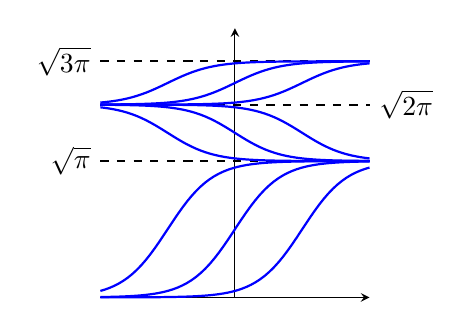
\begin{tikzpicture}
                \begin{axis}[
                        width=5cm,
                        height=5cm,
                        xmin=-2, xmax=2,
                        ymin=0, ymax=3.5,
                        axis lines=middle,
                        xtick=\empty,
                        ytick=\empty,
                        clip=false,
                        domain=-2:2,
                        samples=60
                    ]
                    \addplot[black, thick, dashed] {1.7724};
                    \addplot[black, thick, dashed] {2.5066};
                    \addplot[black, thick, dashed] {3.0699};

                    \node[anchor=east] at (axis cs:-2, 1.7724) {\(\sqrt{\pi}\)};
                    \node[anchor=east] at (axis cs:-2, 3.0699) {\(\sqrt{3\pi}\)};

                    \node[anchor=west] at (axis cs:2, 2.5066) {\(\sqrt{2\pi}\)};

                    \addplot[blue, thick] {1.7724 / (1 + exp(-3*(x+1)))};
                    \addplot[blue, thick] {1.7724 / (1 + exp(-3*x))};
                    \addplot[blue, thick] {1.7724 / (1 + exp(-3*(x-1)))};

                    \addplot[blue, thick] {1.7724 + 0.7342 / (1 + exp(3*(x+1)))};
                    \addplot[blue, thick] {1.7724 + 0.7342 / (1 + exp(3*x))};
                    \addplot[blue, thick] {1.7724 + 0.7342 / (1 + exp(3*(x-1)))};

                    \addplot[blue, thick] {2.5066 + 0.5633 / (1 + exp(-3*(x+1)))};
                    \addplot[blue, thick] {2.5066 + 0.5633 / (1 + exp(-3*x))};
                    \addplot[blue, thick] {2.5066 + 0.5633 / (1 + exp(-3*(x-1)))};
                \end{axis}
            \end{tikzpicture}
\end{center}
\end{snippetexample}

\end{document}
